\section{Giới thiệu (Introduction)}

\subsection{Bối cảnh và vấn đề}

Trong những năm gần đây, phương tiện bay không người lái (Unmanned Aerial Vehicle -- UAV) được quan tâm trong nhiều bài toán như giám sát, khảo sát, cứu hộ và vận chuyển hàng hóa. So với phương tiện mặt đất, UAV có khả năng di chuyển linh hoạt trong không gian ba chiều và tiếp cận những khu vực khó đi lại. Tuy nhiên, để thực hiện nhiệm vụ vận chuyển một cách tự động, UAV cần có khả năng xác định chính xác vị trí hạ cánh, tiếp cận vật thể và thao tác với hàng hóa mà không cần người điều khiển trực tiếp.

% TODO: Chèn hình minh họa bài toán tổng thể: UAV tiếp cận bãi đáp ArUco,
% hạ cánh, gắp hộp hàng và cất cánh trở lại.
\begin{figure}[H]
  \centering
  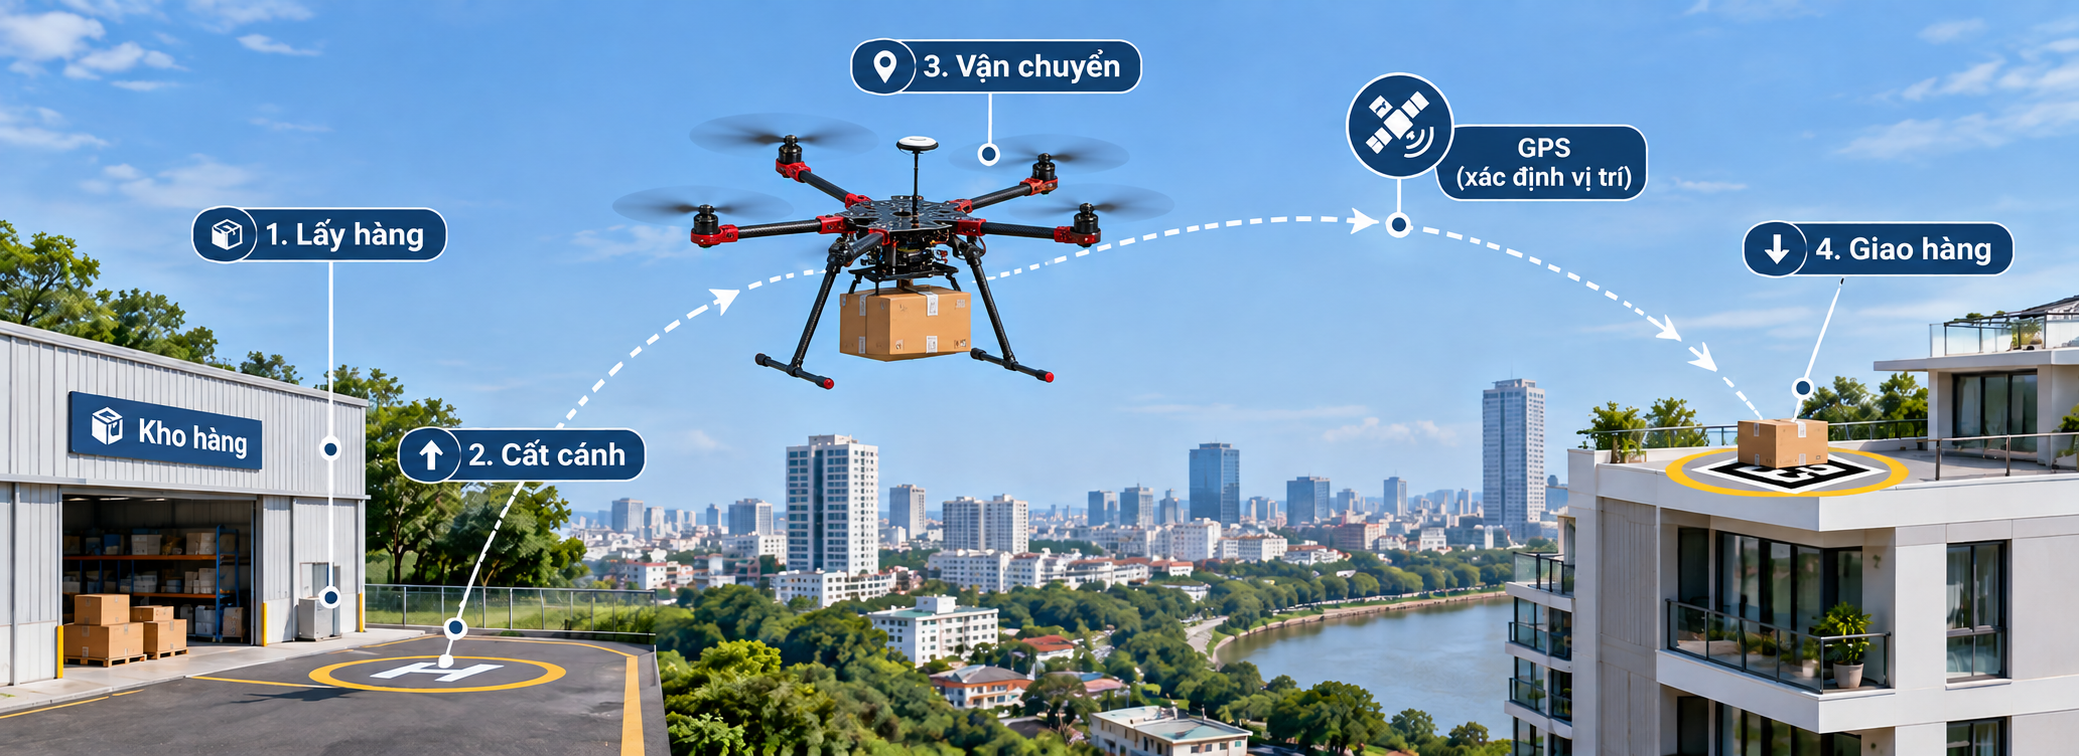
\includegraphics[width=1.0\textwidth]{images/01-drone-deli-pipeline.png}
  \caption{Quy trình nhiệm vụ hạ cánh và gắp hàng tự động}
  \label{fig:quy-trinh-nhiem-vu}
\end{figure}

Một khó khăn quan trọng của bài toán là sai số định vị khi UAV hạ cánh. Tín hiệu GPS thông thường có thể không đủ chính xác đối với một bãi đáp nhỏ, đặc biệt khi môi trường có vật cản hoặc tín hiệu bị che khuất. Vì vậy, đề tài sử dụng camera hướng xuống và mã ArUco đặt trên bãi đáp để tạo ra thông tin vị trí tương đối giữa UAV và mục tiêu. Sau khi hạ cánh, UAV cần kích hoạt cơ cấu gắp để giữ kiện hàng, sau đó cất cánh trở lại mà vẫn duy trì được sự ổn định khi mang tải.



\subsection{Mục tiêu}

Mục tiêu của đồ án là thiết kế và triển khai một hệ thống UAV bốn cánh có khả năng tự động hạ cánh trên bãi đáp được đánh dấu bằng ArUco, gắp kiện hàng và cất cánh lại trên nền tảng Raspberry Pi 5, ROS 2 và PX4.

Các mục tiêu cụ thể gồm:
\begin{itemize}
  \item Xây dựng hệ thống phát hiện mã ArUco từ camera hướng xuống và ước lượng vị trí, hướng tương đối giữa UAV với bãi đáp.
  \item Thiết kế bộ điều khiển hạ cánh dựa trên sai số vị trí và hướng thu được từ hệ thống thị giác.
  \item Tích hợp Raspberry Pi 5 với PX4 thông qua ROS 2 và giao tiếp uXRCE-DDS ở chế độ Offboard.
  \item Thiết kế và điều khiển cơ cấu gripper bằng servo để gắp kiện hàng có khối lượng mục tiêu lớn nhất 1 kg.
  \item Xây dựng máy trạng thái điều phối toàn bộ chu trình Landing--Pickup--Takeoff và các trạng thái xử lý lỗi cơ bản.
  \item Đánh giá hệ thống thông qua độ chính xác hạ cánh, tỷ lệ phát hiện marker, tỷ lệ gắp hàng thành công và thời gian hoàn thành nhiệm vụ.
\end{itemize}

\subsection{Phạm vi}

Đồ án tập trung vào một UAV quadrotor khung S500 được trang bị Raspberry Pi 5, flight controller chạy PX4, camera hướng xuống và cơ cấu gripper điều khiển bằng servo. Mã ArUco được đặt cố định trên bãi đáp và được sử dụng làm mốc định vị tương đối trong giai đoạn tiếp cận và hạ cánh.

Phần mềm được triển khai trên ROS 2, trong đó Raspberry Pi 5 đảm nhiệm thu nhận và xử lý ảnh, ước lượng pose marker, tính toán sai số điều khiển và điều phối nhiệm vụ. Đồ án xét các vật thể gắp có hình dạng và khối lượng nằm trong giới hạn của cơ cấu gripper. Các thử nghiệm được thực hiện trong điều kiện có kiểm soát, với tốc độ bay thấp và không xét đến bài toán tránh vật cản động hoặc lập bản đồ môi trường toàn cục.

\subsection{Đóng góp của đồ án}

Các nội dung chính của đồ án gồm:
\begin{itemize}
  \item Xây dựng pipeline một camera 2D để phát hiện ArUco và cung cấp thông tin pose phục vụ hạ cánh chính xác.
  \item Tích hợp thuật toán điều khiển hạ cánh với PX4, ROS 2 và Raspberry Pi 5 trên một hệ thống UAV thực.
  \item Thiết kế cơ cấu và quy trình điều khiển gripper phù hợp với chu trình hạ cánh, gắp hàng và cất cánh.
  \item Xây dựng máy trạng thái cho nhiệm vụ tự động và đưa ra các tiêu chí đánh giá định lượng cho từng giai đoạn.
\end{itemize}

\subsection{Cấu trúc luận văn}

Luận văn được tổ chức thành năm chương. 
Chương 1 giới thiệu bối cảnh, mục tiêu, phạm vi và các đóng góp của đồ án. 
Chương 2 trình bày kiến thức nền tảng về UAV quadrotor, camera, ArUco, ước lượng pose, điều khiển và các công trình liên quan. 
Chương 3 mô tả kiến trúc phần cứng, kiến trúc phần mềm và phương pháp thiết kế hệ thống. 
Chương 4 trình bày thiết lập thực nghiệm, kết quả đo lường và phân tích các trường hợp thành công hoặc thất bại. Cuối cùng, Chương 5 tổng kết kết quả đạt được và đề xuất hướng phát triển tiếp theo.
